\documentclass[a4paper,12pt]{article}
\usepackage{authblk}
\usepackage{graphicx}
\usepackage{amsmath}
\usepackage[backend=biber, style=apa]{biblatex}
\usepackage{hyperref} 
\usepackage{setspace}
\usepackage{geometry}
\usepackage{tabularx}
\usepackage{caption}
\usepackage{booktabs}
\usepackage{array}
\usepackage{float}
\usepackage{subcaption}

\addbibresource{reference_nutrient_bibtex.bib} 

% Title and author information
\title{Assessing Soil Nutrient Dynamics and Their Impacts on Crop Yields: A Case Study of Janaki Rural Municipality, Banke, Nepal }

\author[1]{Rasila Gautam*}
\author[1]{Bishwa Prakash Puri}
\author[1]{Bhupendra Devkota}
\author[1,2]{Tirtha Raj Adhikari}


\author[ ]{Janak Lal Nayava}

\affil[1]{College of Applied Sciences-Nepal, Tribhuvan University, Kathmandu, Nepal}
\affil[2]{Central Department of Hydrology and Meteorology, Tribhuvan University, Kirtipur, Nepal}
\affil[*]{Correspondence Author: \texttt{rasilagautam2@gmail.com}}

\date{}  


\begin{document}
\maketitle
\begin{abstract}


Nepal's diverse climate, spanning from subtropical lowlands to arctic high mountains, poses significant challenges for its predominantly agriculture-dependent population. This study examines the impact of climate variability on agricultural productivity and food security in Banke, Nepal, over the period 1990--2020. Analysis of long-term climatic data revealed a minor but steady increase in average temperature (0.0946\,°C per year), a significant upward trend in sunshine hours (15.15 hours per year, $R^2 = 0.3125$), and a modest annual rise in accumulated rainfall (approximately 1.94\,mm per year). Correlation analysis indicates that sunshine hours have a significant positive effect on crop yield ($r = 0.417$, $p = 0.017$), whereas rainfall and temperature exhibit weaker, statistically non-significant relationships. A linear regression model incorporating these variables explained 24.2\% of the variation in crop yield. Additionally, the region’s agricultural profile is characterized by a high reliance on monoculture, limited crop diversification, and minimal institutional support despite generally sufficient food production. Shifts in cropping calendars and irrigation practices—most notably, the higher yields achieved under year-round irrigation compared to rainfed systems—further underscore farmers' adaptive responses to climate uncertainties. These findings highlight the dominant role of solar radiation in driving crop productivity and underscore the need for integrated, climate-resilient strategies to ensure long-term agricultural sustainability and food security.


\noindent \textbf{Keywords:} Climate variability, Agricultural productivity, Food security, Irrigation and Crop yield, Climate change adaptation


\end{abstract}

\section{Introduction}
Agriculture in Nepal is based on subsistence farming for the majority of the population and this can never be underestimated. The growth of Nepalese agriculture was low and very vulnerable in recent decades  \parencite{gyawaliOverviewAgricultureNepal2021}. Despite the excellent production potential, farmers continue to face enormous challenges. Poverty, land degradation, low agricultural productivity, wrong use of budget and subsidies, shortage. The development of agriculture was hindered by the number of agricultural inputs, poor government support, etc. The challenge of maintaining food security was the simultaneous growth of the population on the one hand and the reduction of cultivated land on the other \parencite{gyawaliOverviewAgricultureNepal2021}.
In Nepal's agriculture, coarse grains and pulses are crucial for food and nutritional security, the nitrogen economy, and job possibilities  They serve a dual purpose in Nepal, playing a significant role in both trade and survival. Coarse grains and pulses are important components of the Nepalese diet, providing much-needed nutrients to the common people(Db et al., 2014). 
1.1.2.2 Current Scenario:
Out of Nepal's total land area of 147,181 square kilometers, cultivated agricultural land makes up 21\% and uncultivated agriculture land makes 7\% of total land use (MOALD, 2020). In the last few years, Nepal's agricultural growth has accelerated significantly. The remaining 75.9\% of farmers do subsistence farming, while just 25.1\% engage in commercial farming. Although grain, cash crop, and pulse output has greatly improved over the past few years, it still isn't enough to feed the growing population (Simkhada 2019). The majority of farms in Nepal (53\%) are small-scale, with landholdings of no more than 0.5 hectares, while the remaining 20\% are large-scale, with landholdings of more than 1 hectares. More than one-fourth (26\%) of agricultural landowners in Nepal are women (FAQ 2020). 

\subsubsection{Agricultural Land Use}
The land problem is one of the most common concerns of all nations. In Nepal, cultivation is still unplanned and uncontrolled and there has been a tremendous shift in land use from agriculture to other purposes where cultivation is more flourishing in the Terai region of Nepal. Demand for land-intensive crops is increasing in the rapidly developing South Asian region, including Nepal (Timilsina et al., 2019). A recent FRTC study (2019) showed that the cultivated land is 21.88 percent of the entire country. This shows the recent growth of cultivated area in Nepal. The average land holding per family in Nepal is less than 0.68 ha (CBS, 2013), which has gradually decreased over the last three decades. In addition, agricultural land is regularly fragmented for several reasons, especially in the Terai zone of Nepal (Shrestha, 2011). Land use for temporary and permanent crops grown show an opposite trend, with permanent crops increasing and temporary crops decreasing. The number of land parcels has significantly increased, supporting the fact about increased land fragmentation trend in Nepal.
Today's growth in crop production in Nepal is due only to increased production area, however, the trend is to reduce agricultural land especially in the Terai due to urbanization and land fragmentation between 1989 and 2016 is a major obstacle to achieving food security in the country. So, the need is great increase the efficiency of land use to solve the problem of increasing food demand (Timilsina et al., 2019). 
2.5 Fertilizers in Agriculture:
More nutrients in the form of chemical fertilizers are needed to maximize high grain yields and meet the growing food demand of the majority of Nepal's population (Lamichhane et al., 2022). Chemical fertilizers are rich in nutrients; therefore, only a small amount is needed for productivity (Han et al 2016). A study carried by (Baral et al., 2020) in Nepalgunj, Banke found that different farm types, varietals, and irrigation systems have quite different fertilizer application procedures. Farmers utilized 55:39:15 kg N: P2O5:K2O ha-1 on average. The sources of these nutrients were urea, DAP, and MOP. Farmers' fertilizer usage was shown to be unbalanced overall. Amounts of N fertilizer used per hectare ranged from 0 kg to 138 kg. Compared to medium (57 kg ha-1) and small (41 kg ha-1) farmers, large farmers submitted applications at a greater rate (73 kg ha-1) (Baral et al., 2020). Although farmers have reported using more inorganic fertilizer over the previous five years, actual usage is still less than what the government advises. According to Takeshima et al. (2016), large farmers often use more nitrogen fertilizer than medium-sized and small-sized farms, perhaps because they have more financial resources and fewer organic inputs available.
2.8 Agricultural Land Use:
Demand for land-intensive crops is increasing in the rapidly developing South Asian region, including Nepal (Timilsina et al., 2019). A recent FRTC study (2019) showed that the cultivated land is 21.88 percent of the entire country. This shows the recent growth of cultivated area in Nepal. The average land holding per family in Nepal is less than 0.68 ha (CBS, 2013), which has gradually decreased over the last three decades. In addition, agricultural land is regularly fragmented for several reasons, especially in the Terai zone of Nepal (Shrestha, 2011). 
Today's growth in crop production in Nepal is due only to increased production area, however, the trend is to reduce agricultural land especially in the Terai due to urbanization and land fragmentation between 1989 and 2016 is a major obstacle to achieving food security in the country. So, the need is great increase the efficiency of land use to solve the problem of increasing food demand (Timilsina et al., 2019). According to (Devkota et al., 2023) Nepalgunj had the highest coverage of agricultural areas; the proportion of agricultural areas in Nepalgunj was 95.38\% (83.51 km2), 90.03\% (78.82 km2) and 89.77\% (78.6 km2) in the year 1990, 2000 and 2010 respectively.

This study focuses on understanding the impact of climate change on agriculture and food security in Janaki Rural Municipality, Banke, with a particular emphasis on nutrient dynamics, fertilizer use, and land-use changes. Climate change has disrupted soil nutrient availability and fertilizer efficiency, thereby affecting crop yields. Additionally, shifting land-use patterns, such as the conversion of agricultural lands for non-agricultural purposes, have further diminished the area available for cultivation. Analyzing the status of soil fertility and irrigation, along with changes in cultivated land over the past 20 years, is critical to addressing the challenges posed by climate change. By evaluating these factors and their relationship to food security, the study aims to provide insights that will guide sustainable agricultural practices and strategic planning to mitigate climate impacts on food production in the region.

1.1.5.2 Fertilizers/ Nutrient:
More nutrients in the form of chemical fertilizers are needed to maximize high grain yields and meet the growing food demand of the majority of Nepal's population (Lamichhane et al., 2022).One of the most important inputs for agricultural output is fertilizer. According to APP, higher fertilizer usage accounts for nearly half of the incremental production and it has been determined that a key contributing factor in the poor production and productivity of agricultural commodities is farmers' inadequate access to seed and fertilizer (Pandey et al., 2017). Chemical fertilizers are used to correct plant nutrient deficiencies, providing large amounts of nutrients to help plants withstand stress, maintain optimal soil fertility, and improve crop quality. Because the nutrients in chemical fertilizers are already soluble in water, they promote the rapid development of plants and are effective quickly and effectively. Chemical fertilizers are rich in nutrients; therefore, only a small amount is needed for productivity (Han et al 2016). Chemical fertilizers have been found to increase yields for a few years, but are ineffective in the long term and contribute to soil degradation. Chemical fertilizers accelerate the decomposition of organic matter in the soil, which weakens the soil structure and reduces soil aggregation. As a result, nutrients are easily lost from the soil through fixation, leaching and gassing, reducing the effectiveness of fertilizers (Alimi et al 2007). Higher doses of chemical fertilizers not only reduce the microbial population (Gruhn et al 2000) but also causes an imbalance of soil nutrients, which can lead to soil acidity and reduced yields (Ojeniyi 2002).



\section{Study area, Data and Methods}
\subsection{Study Area}



The study area of this research is Janaki Rural Municipality of Nepalgunj, Banke (Figure ). The elevation of Janaki Rural Municipality is 165m above sea level. It is bordered by Nepalgunj Sub Metropolitan in the east, Kohalpur Municipality in the north, Khajura Rural Municipality in the west, and India in the south (Janaki Rural Municipality, 2075). The region experiences a temperate climate, characterized by flat terrain. According to the meteorological department records, the average annual rainfall is 1445.58 mm. The maximum recorded temperature reaches 46°C, while the minimum temperature is 4.5°C (Janaki Rural Municipality, 2075). Farming is the primary income source for most families. Of the 5,063 ha of cultivable land, only 2,532 ha is utilized, with 1,798 ha as farmland and 774 ha as upland.

In Janaki Rural Municipality, 1,294 households own less than 0.167 ha, 1,222 own 0.2–0.33 ha, 2,338 own 0.37–0.67 ha, 1,512 own 0.7–1 ha, and 973 own more than 20 ha, while 52 households are landless. Of the land, only 321 ha is irrigated year-round, and 1,871 ha lack irrigation. The municipality has 50 ponds, some used for irrigation. Despite abundant arable land, limited irrigation and technological support prevent commercial farming, leading many to rely on India for food supplies (Janaki Rural Municipality, 2075).

Janaki Rural Municipality consists of six wards in total, out of which three wards were randomly sampled and included in the research study as follows (Table \ref{tab:study_area}): 

\begin{table}[h]
\centering
\caption{Study Area with elevation and coordinates}
\label{tab:study_area}
\resizebox{\textwidth}{!}{
\begin{tabular}{|c|l|c|l|}
\hline
\textbf{S.N.} & \textbf{Study Location} & \textbf{Elevation (m)} & \textbf{Coordinates} \\ \hline
1 & Janaki Rural Municipality – 01, Saigaun & 164 & 28°02'42"N 81°34'05"E \\ \hline
2 & Janaki Rural Municipality – 03, Indrapur & 172 & 28°05'02"N 81°36'20"E \\ \hline
3 & Janaki Rural Municipality – 04, Khajura Khurda & 163 & 28°06'26"N 81°36'00"E \\ \hline
\end{tabular}
}
\end{table}

Source: (Janaki Rural Municipality, 2075)

\subsection{Methods of Data Collection}

\subsubsection{Primary Source of Data}
A comprehensive household survey and intensive field research were carried out in Janaki Rural Municipality's wards 01, 03, and 04, which included a total of 47 villages. Structured interviews and direct observations were used to collect data on agriculture, irrigation, food security, and perceptions of climate change. Village sample sizes were assessed using household ratios, and then systematic sampling was conducted.

\subsubsection{Secondary Source of Data}
The secondary data were taken from literature reviews relevant to the research topic, where the majority of reviews were collected from desk studies, i.e., the internet. Various knowledge and data were achieved through reference books, recently published national newspapers, international journals, reports, records, past literature, reviews of various websites, and so on.

\subsubsection{Sampling Frame}
Stratified random sampling was utilized in a survey conducted in Janaki Rural Municipality, where wards 1, 3, and 4 were chosen by lottery out of six wards. Villages were sampled proportionally, whereas households within each village were systematically selected based on municipality-provided household data. Janaki Rural Municipality, divided into six wards, had wards 1, 3, and 4 selected for the study using a lottery method. Ward 1 includes 5 villages, while wards 3 and 4 have 21 villages each, as identified by an internal survey in 2075 B.S. Villages were proportionately sampled through stratified random sampling to ensure diversity and minimize sampling errors. Observations were also conducted to gather information on homes within each village.

The details of the household distribution are provided in Table \ref{tab:household_distribution}.

\begin{table}[h]
\centering
\caption{Household Distribution by Ward}
\label{tab:household_distribution}

\begin{tabular}{|c|c|c|}
\hline
\textbf{Ward} & \textbf{Household} & \textbf{Soil Sample} \\ \hline
1 & 1242 & 8 \\ \hline
3 & 1929 & 8 \\ \hline
4 & 1050 & 8 \\ \hline
\textbf{Total} & 7391 & 24 \\ \hline
\end{tabular}
\end{table}



\subsection{Sample Size Determination}
Total household population was obtained from the report obtained from Janaki Rural Municipality from the internal survey conducted in 2075 B.S. The sample size of the population to conduct the questionnaire survey was calculated at a 95\% confidence level using the formula:

\[
n = \frac{N \cdot z^2 \cdot p \cdot q}{(N - 1) \cdot e^2 + z^2 \cdot p \cdot q}
\]

\textbf{Source:} Dahal, 2021

Where:
\begin{itemize}
    \item $n$ = Sample size
    \item $N$ = Total number of households of selected wards
    \item $z$ = Confidence level at 95\%, $z = 1.96$
    \item $p$ = Expected rate of occurrence = 0.9
    \item $q$ = $1 - p = 0.1$ (expected rate of non-occurrence)
    \item $e$ = Degree of error = 0.05
\end{itemize}

\[
n = \frac{4221 \cdot (1.96)^2 \cdot 0.9 \cdot 0.1}{(4221 - 1) \cdot (0.05)^2 + (1.96)^2 \cdot 0.9 \cdot 0.1}
\]

\[
n = 133.9 \approx 134
\]

The selection of households from each ward was calculated using the following formula:

\[
n_h = \frac{N_h}{N} \cdot n
\]

\textbf{Source:} Dahal, 2021

Where:
\begin{itemize}
    \item $n_h$ = Sample size for each ward
    \item $N_h$ = Population size of each ward
    \item $N$ = Total population size = 4221
    \item $n$ = Total sample size = 134
\end{itemize}

\subsection{Sample Size of Selective Wards}

The sample size for each ward is calculated as follows:

\begin{table}[h]
\centering
\caption{Sample Size of Selective Wards}
\label{tab:sample_size_wards}
\begin{tabular}{|c|c|c|c|}
\hline
\textbf{Ward} & \textbf{$N_h$} & \textbf{$N_h / N$} & \textbf{$N_h / N \cdot n$} \\ \hline
1 & 1242 & 0.29 & 39 \\ \hline
3 & 1929 & 0.457 & 61 \\ \hline
4 & 1050 & 0.249 & 33 \\ \hline
\textbf{Total} & 4221 & & 134 \\ \hline
\end{tabular}
\end{table}

\subsection{Sample Size of Selective Villages}

The sample size for selective villages of ward 1 (Saigaun) is shown in Table \ref{tab:sample_size_village_ward1}:

\begin{table}[h]
\centering
\caption{Sample Size of Selective Village of Ward 1 (Saigaun)}
\label{tab:sample_size_village_ward1}
\resizebox{\textwidth}{!}{
\begin{tabular}{|c|c|c|c|}
\hline
\textbf{Village} & \textbf{Household Number} & \textbf{Sample Size} & \textbf{Sample Size Cumulated} \\ \hline
3 & 414 & 13 & 13 \\ \hline
5 & 331 & 10.39 & 10 \\ \hline
\textbf{Total} & 1242 & 39 & 39 \\ \hline
\end{tabular}
}
\end{table}

The sample size for selective villages of ward 3 (Indrapur) is shown in Table \ref{tab:sample_size_village_ward3}:

\begin{table}[h]
\centering
\caption{Sample Size of Selective Village of Ward 3 (Indrapur)}
\label{tab:sample_size_village_ward3}
\resizebox{\textwidth}{!}{
\begin{tabular}{|c|c|c|c|}
\hline
\textbf{Village} & \textbf{Household Number} & \textbf{Sample Size} & \textbf{Sample Size Cumulated} \\ \hline
1 & 127 & 4.02 & 4 \\ \hline
3 & 85 & 2.69 & 3 \\ \hline
19 & 149 & 4.71 & 5 \\ \hline
\textbf{Total} & 1929 & 61 & 61 \\ \hline
\end{tabular}
}
\end{table}

The sample size for selective villages of ward 4 (Khajura Khurda) is shown in Table \ref{tab:sample_size_village_ward4}:

\begin{table}[h]
\centering
\caption{Sample Size of Selective Village of Ward 4 (Khajura Khurda)}
\label{tab:sample_size_village_ward4}
\resizebox{\textwidth}{!}{
\begin{tabular}{|c|c|c|c|}
\hline
\textbf{Village} & \textbf{Household Number} & \textbf{Sample Size} & \textbf{Sample Size Cumulated} \\ \hline
3 & 50 & 1.57 & 2 \\ \hline
10 & 62 & 1.95 & 2 \\ \hline
15 & 87 & 2.73 & 3 \\ \hline
\textbf{Total} & 1050 & 33 & 33 \\ \hline
\end{tabular}
}
\end{table}

\subsubsection{Data Collection and Calculation}
The initial step was to collect the necessary data and the extractions of pertinent factors in order to accomplish the main goal of the examining the production trend and climatic scenario along with other variables and their correlation in the research area. Subsequently, these factors were scrutinized to identify their inter relationship and trends. The data used for this analysis were sourced from a variety of outlets, encompassing both primary and secondary data, along with ancillary data, to ensure a comprehensive and high-quality analysis. The process of gathering data involved accessing a rich pool of information from government reports, academic literature, and books, thereby offering a more expansive context and historical viewpoint for the research.
Moreover, adding information from trustworthy websites and internet sources improved the dataset's currency and depth. This diverse approach to data collection ensured the study's dependability and thoroughness while also enhancing its richness. Important contextual facts were acquired from reputable organizations including DHM, and MOALD. These details contributed to a thorough understanding of the issues influencing the research region. The primary, secondary, and auxiliary sources were all covered by this comprehensive data collection methodology. These many techniques for gathering data have enabled this thesis to get an accurate outcome to address the objectives.
IBM SPSS statistical 27 tool and Microsoft Excel was used to carry statistical analysis. 

\paragraph{Pearson Correlation Coefficient}
Pearson correlation coefficient is used for yield, sunshine hour, and accumulated rainfall to calculate the linear relationship between them before simple linear regression, where total yield is the dependent variable, and sunshine radiation, accumulated rainfall, and average temperature are the independent variables.

Pearson correlation coefficient (r) is a popular method for calculating a linear correlation. The degree and direction of the relationship between two variables are indicated by the correlation coefficient, which has a range of -1 to 1 Turney2022. 

A perfect positive correlation ($r = 1$) means that as one variable rises, the other rises in proportion.
A complete negative correlation ($r = -1$) means that as one variable rises, the other falls proportionately.
($r = 0$) indicates no linear correlation between the variables.

The formula for the Pearson correlation coefficient (r) between two variables (X) and (Y) with (n) data points is given by:
\[
r = \frac{n \sum_{i=1}^{n} (x_i - \bar{x})(y_i - \bar{y})}{\sqrt{\sum_{i=1}^{n} (x_i - \bar{x})^2} \sqrt{\sum_{i=1}^{n} (y_i - \bar{y})^2}}
\]

Where:
\begin{itemize}
    \item $X_i$ and $Y_i$ are individual data points for variables X and Y, respectively.
    \item $\bar{X}$ and $\bar{Y}$ are the means (average) of the variables X and Y, respectively.
    \item $\sum$ represents the summation symbol, indicating that you need to sum the quantities inside it across all data points.
\end{itemize}

Source: Turney2022

\paragraph{Simple Linear Regression Analysis}
Simple linear regression analysis is used in this study to establish the relationship between the dependent variable (Yield) and independent variables (climate data). This statistical technique allows for the examination of how changes in one variable (independent variable) affect changes in another variable (dependent variable) through the estimation of a linear relationship between them Mali2023.

The equation of simple linear regression is:
\[
Y_i = \beta_0 + \beta_1 X_i + \epsilon
\]

Where:
\begin{itemize}
    \item $Y_i$ represents the dependent variable; $X_i$ represents the independent variable.
    \item The intercept, denoted by $\beta_0$, indicates the value of $Y$ when $X$ equals 0.
    \item $\beta_1$ is the slope of the line, representing the change in $Y$ for a unit change in $X$.
    \item $\epsilon$ represents the error term, accounting for the differences between the observed and predicted values.
\end{itemize}

\paragraph{T-test}
The T-test is used to compare the average yields (in kilograms per hectare) of two groups categorized by different irrigation methods: year-round irrigation and rainfed irrigation during the monsoon season.

\begin{itemize}
    \item \textbf{Year-round Irrigation:} Agricultural plots where irrigation is consistently applied throughout the year.
    \item \textbf{Rainfed Irrigation:} Agricultural plots relying solely on rainfall during the monsoon season for irrigation.
\end{itemize}

Statistical software package (SPSS) is used for analysis. The t-test is performed to compare the average yields between the two irrigation groups. The significance level ($\alpha$) is set a priori to 0.05.

\[
H_0: \text{There is no difference in yields between the two groups.}
\]
\[
H_1: \text{There is a difference in yields between the two groups.}
\]

A statistical test for comparing the means of two groups is called a t-test. It is frequently employed in hypothesis testing to ascertain whether two groups are distinct from one another or whether a procedure or treatment genuinely affects the population of interest Bevans2020.

The t-test statistic is given by the formula:
\[
t = \frac{\overline{x_1} - \overline{x_2}}{\sqrt{S^2 \left( \frac{1}{n_1} + \frac{1}{n_2} \right)}}
\]

Where:
\begin{itemize}
    \item $\overline{x_1}$ and $\overline{x_2}$ represent the means of the two samples.
    \item $S^2$ represents the pooled variance of the two samples.
    \item $\frac{1}{n_1} + \frac{1}{n_2}$ represents the sizes of the two samples.
\end{itemize}

Source: Student1908, Zabell2008

\paragraph{Index Model}
An index model determines the index value for every unit area and uses those values to create a ranking map. An index model and a binary model are comparable in that they both rely on overlay operations for data processing and require multicriteria assessment. However, an index model generates an index value, not just a yes or no, for every unit area \cite{OneStopGIS2020}.

Two tiers of evaluation are applied to certain variables:
\begin{itemize}
    \item Considering relative significance and weighing.
    \item Values that are seen are assessed and assigned scores OneStopGIS2020.
\end{itemize}

\paragraph{Climate Change and Production Trend Analysis}

The simple linear regression analysis was carried out using IBM SPSS Statistical 27 tool to identify the relationship between the dependent and independent variables. In this data, production yield data is the dependent variable, and climatic variables such as accumulated precipitation data, average temperature, and sunshine radiation are the independent variables.

Initially, the correlation between these variables was computed, and afterward, the linear relationship between climate variables (sunshine hours, temperature, and rainfall) and yield was analyzed through simple linear regression analysis.

\paragraph{Climate Change Trend}

Three variables for climate change were studied, which included Accumulated Rainfall, Average Temperature, and Sunshine hours of the study area for the last thirty years, from 1990 to 2021. The data were obtained from the Department of Hydrology and Meteorology. Excel was used for plotting the linear trend graph.

\paragraph{Climate Change Perception}

An index model has been used to evaluate the perception of farmers towards climate change and its impact on agricultural production. Understanding of climate change and its impacts is deeply rooted in the perception of farmers towards climate change. A total of 134 respondents were asked to give their opinion on the following statement.

A three-point scale was used with the frequency of agreement/approval as +1, frequency of disagreement/disapproval as -1, and "don’t know/absent" was given as 0.

The following formula by Dahal (2021) has been used for calculating the index for binary variables:

\[
\text{INDEX} = \frac{FA(+1) + FDA(-1) + FDK(0)}{N}
\]

Where:
\begin{itemize}
    \item $FA$: Frequency of agreement/approval
    \item $FDA$: Frequency of disagreement/disapproval
    \item $FDK$: Frequency of "don’t know/absent"
    \item $N$: Total number of respondents = 134
\end{itemize}

For variables with multiple categories, the following formula has been used to calculate the index based on a data normalization technique (Nguyen 2019):

\[
\text{INDEX} = \frac{(\text{Max value} - \text{Min value}) \times X}{(\text{Max value} + \text{Min value}) \times \text{Max value}}
\]

Where $X$ is the value of a particular category.

\section{Results and Discussion}

\subsection{Seasonal Temperature Trends}

Figures\ref{fig:Pre_monsoon_temperature_trends, fig:Monsoon_temperature_trends, fig:Post_monsoon_temperature_trends, fig:Winter_temperature_trends, fig:Annual_temperature_trends}  display temperature trend analyses based on three primary factors: temperature categories (Tavg, Tmax, Tmin), geographic regions (Himalayas, High Mountain, Middle Mountain, Siwalik, Tarai, and the entire Koshi Basin), and seasonal classifications (Monsoon, Post-monsoon, Pre-monsoon, Winter, and annual trends) across various decades. The trends reveal substantial variability influenced by decade, temperature type, physiographic region, and seasonal attributes.

\subsection*{Pre-monsoon}

\begin{figure}[H] 
  \centering
  \includegraphics[width=0.9\textwidth]{images/simple_plots_Premonsoon_Trend.png}  
  \caption{Pre-monsoon temperature trends across the time intervals (a) 1962–1971, (b) 1972–1981, (c) 1982–1991, (d) 1992–2001, (e) 2002–2011, (f) 2012–2021, and (g) 1962–2022.} 
  \label{fig:Pre_monsoon_temperature_trends}  
\end{figure}

Pre-monsoon season reveals overall cooling trends in the 1962-1971 decade except in Himalaya regions, similar cooling trend from 1972 to 1981, and later decade experience a warming trend except maximum and average temperature shows cooling trend in 2012-2021 (Figure \ref{fig:Pre_monsoon_temperature_trends}) For the overall period from 1962 to 2022, only the Siwalik region demonstrates a cooling trend; all other regions display warming trends, particularly the Himalayan region, which shows a higher rate of warming at 0.02$^\circ$C/year.  

\subsection*{Monsoon}
During the Monsoon season (Figure \ref{fig:Monsoon_temperature_trends}), temperature fluctuations have accelerated in recent decades, particularly from 2012 to 2021, with significant warming observed in average and minimum temperatures, while maximum temperatures predominantly show a cooling trend. Overall, from 1962 to 2022, the Monsoon season reflects a cooling trend across the various regions.

\begin{figure}[H] 
  \centering
  \includegraphics[width=0.9\textwidth]{images/simple_plots_Monsoon_Trend.png}  
  \caption{Monsoon temperature trends across the time intervals (a) 1962–1971, (b) 1972–1981, (c) 1982–1991, (d) 1992–2001, (e) 2002–2011, (f) 2012–2021, and (g) 1962–2022.} 
  \label{fig:Monsoon_temperature_trends}  
\end{figure}

\subsection*{Post-monsoon}

\begin{figure}[H] 
  \centering
  \includegraphics[width=0.9\textwidth]{images/simple_plots_Postmonsoon_Trend.png}
  \caption{Post-monsoon temperature trends across the time intervals (a) 1962–1971, (b) 1972–1981, (c) 1982–1991, (d) 1992–2001, (e) 2002–2011, (f) 2012–2021, and (g) 1962–2022.}
  \label{fig:Post_monsoon_temperature_trends}  
\end{figure}

A cooling trend is evident in the post-monsoon period from 1962 to 1981 (Figure \ref{fig:Post_monsoon_temperature_trends}), followed by a notable warming trend that has intensified in recent decades.

\subsection*{Winter}

\begin{figure}[H] 
  \centering
  \includegraphics[width=0.9\textwidth]{images/simple_plots_Winter_Trend.png}  
  \caption{Winter temperature trends across the time intervals (a) 1962–1971, (b) 1972–1981, (c) 1982–1991, (d) 1992–2001, (e) 2002–2011, (f) 2012–2021, and (g) 1962–2022.} 
  \label{fig:Winter_temperature_trends}  
\end{figure}


Distinct temperature trends are observed during the Winter season (Figure \ref{fig:Winter_temperature_trends}) across different regions and time periods. Minimum and average temperatures showed warming between 1982–1991 and 2012–2021, while a cooling trend occurred from 1962–1971. Maximum temperatures increased during the 1992–2001 and 2002–2011 decades, with a notable cooling of 0.52$^\circ$C in the High Mountain region from 2012 to 2021. Overall, from 1962 to 2022, the Siwalik region experienced a general cooling trend, while only the High Mountain region exhibited a warming trend.

\subsection*{Annual}

\begin{figure}[H] 
  \centering
  \includegraphics[width=0.9\textwidth]{images/simple_plots_annual_Trend.png}  
  \caption{Annual temperature trends across the time intervals (a) 1962–1971, (b) 1972–1981, (c) 1982–1991, (d) 1992–2001, (e) 2002–2011, (f) 2012–2021, and (g) 1962–2022.} 
  \label{fig:Annual_temperature_trends}  
\end{figure}

Figure \ref{fig:Annual temperature trends} illustrates the annual temperature trends across different regions of the Koshi Basin revealing significant variations over the decades. The first two decades (1962-1981) exhibit an overall cooling trend, with the exception of warming observed in the Himalayan regions, where maximum temperatures increased by 0.02 °C and minimum temperatures rose by 0.04 °C in later decades. The period from 1982 to 2021 predominantly shows a warming trend; however, from 2002 to 2011, the Siwalik region experienced a cooling trend, and in 2012 to 2021, maximum temperatures again exhibited a cooling trend. In overall annual temperature trends in Koshi Basin showed decreasing trend followed by increasing trend similar to study conducted by \textcite{chand_trend_2019} at Narayani Basin Nepal. 


Temporal and spatial analysis of five physiographic regions- Tarai, Siwalik, Middle-mountain, and High-mountain and Himalayas of Koshi Basin presented via Table \ref{tab:spatial_trends}.

\begin{table}[htbp]
  \centering
  \caption{Spatial distribution of temporal trends of temperature for 1962-2022}
  \begin{tabular}{@{}lcccccc@{}}
      \toprule
      Region & Tmax Trend & Tmax p-value & Tmin Trend & Tmin p-value & Tavg Trend & Tavg p-value \\ 
      \midrule
      \textbf{Himalaya} & & & & & & \\ 
      Monsoon & -0.0111 & 0.1672 & -0.0160 & 0.2340 & -0.0135 & 0.1964 \\ 
      Postmonsoon & 0.0114 & 0.1412 & -0.0011 & 0.9435 & 0.0051 & 0.6504 \\ 
      Premonsoon & \textbf{0.0186*} & 0.0115 & 0.0040 & 0.7977 & 0.0113 & 0.3058 \\ 
      Winter & 0.0031 & 0.7077 & -0.0177 & 0.0972 & -0.0073 & 0.4334 \\ 
      \midrule
      \textbf{High Mountain} & & & & & & \\ 
      Monsoon & -0.0038 & 0.5811 & \textbf{-0.023*} & 0.0019 & \textbf{-0.01*} & 0.0062 \\ 
      Postmonsoon & \textbf{0.0233*} & 0.0035 & 0.0128 & 0.1022 & \textbf{0.02*} & 0.0035 \\ 
      Premonsoon & 0.0125 & 0.0845 & \textbf{0.0164*} & 0.0103 & \textbf{0.01*} & 0.0084 \\ 
      Winter & \textbf{0.0317*} & 0.0058 & -0.0088 & 0.2583 & 0.0114 & 0.1407 \\ 
      \midrule
      \textbf{Middle Mountain} & & & & & & \\ 
      Monsoon & \textbf{-0.0122*} & 0.0338 & \textbf{-0.013*} & 0.0076 & \textbf{-0.01*} & 0.0157 \\ 
      Postmonsoon & 0.0032 & 0.5873 & 0.0011 & 0.8304 & 0.0021 & 0.6808 \\ 
      Premonsoon & 0.0071 & 0.2333 & 0.0074 & 0.1586 & 0.0072 & 0.1738 \\ 
      Winter & -0.0004 & 0.9422 & \textbf{-0.021*} & 0.0002 & \textbf{-0.01*} & 0.0466 \\ 
      \midrule
      \textbf{Siwalik} & & & & & & \\ 
      Monsoon & \textbf{-0.0552*} & 0.0000 & \textbf{-0.06*} & 0.0000 & \textbf{-0.06*} & 0.0000 \\ 
      Postmonsoon & -0.0135 & 0.0945 & \textbf{-0.04*} & 0.0000 & \textbf{-0.03*} & 0.0003 \\ 
      Premonsoon & -0.0106 & 0.1916 & \textbf{-0.04*} & 0.0005 & \textbf{-0.03*} & 0.0017 \\ 
      Winter & \textbf{-0.0260*} & 0.0030 & \textbf{-0.10*} & 0.0000 & \textbf{-0.06*} & 0.0000 \\ 
      \midrule
      \textbf{Tarai} & & & & & & \\ 
      Monsoon & \textbf{-0.0183*} & 0.0005 & -0.0215 & 0.0000 & -0.0199 & 0.0000 \\ 
      Postmonsoon & 0.0027 & 0.5809 & -0.0045 & 0.4620 & -0.0009 & 0.8552 \\ 
      Premonsoon & 0.0067 & 0.2577 & 0.0011 & 0.8275 & 0.0039 & 0.4280 \\ 
      Winter & -0.0006 & 0.9121 & -0.0280 & 0.0000 & -0.0143 & 0.0104 \\ 
      \bottomrule
  \end{tabular}
  \label{tab:spatial_trends}
  \begin{flushleft}
    \footnotesize{* Indicates \( p \leq 0.05 \) which denotes significant changes} \\
    
\end{flushleft}
\end{table}




In the five physiographic regions of Koshi Basin, temperature trends display distinct seasonal variations across physiographic regions (Table \ref{tab:spatial_trends}).

In the Himalaya region, a significant warming trend is observed during the pre-monsoon season in Tmax (0.0186, p=0.0115), while other trends remain largely non-significant, including slight cooling in the monsoon (Tmax: -0.0111, p=0.1672; Tmin: -0.0160, p=0.2340) and winter seasons (Tmin: -0.0177, p=0.0972).
The High Mountain region exhibits significant temperature changes across multiple seasons. In the post-monsoon, Tmax and Tavg show strong warming trends (Tmax: 0.0233, p=0.0035; Tavg: 0.0200, p=0.0035), while the monsoon season shows a significant cooling trend in Tmin (-0.0230, p=0.0019). The pre-monsoon season also reflects a notable warming in Tmin (0.0164, p=0.0103) and Tavg (0.0100, p=0.0084), with additional warming in Tmax during winter (0.0317, p=0.0058).
In the Middle Mountain region, a significant cooling trend is observed in the monsoon for both Tmax (-0.0122, p=0.0338) and Tmin (-0.0130, p=0.0076). The winter season also displays significant cooling in Tmin (-0.0210, p=0.0002) and Tavg (-0.0100, p=0.0466), while other seasons show minimal changes.
The Siwalik region experiences substantial cooling across all seasons, particularly in the monsoon, where strong cooling trends are present in Tmax (-0.0552, p=0.0000), Tmin (-0.0600, p=0.0000), and Tavg (-0.0600, p=0.0000). Similarly, significant cooling trends persist in the winter season (Tmax: -0.0260, p=0.0030; Tmin: -0.1000, p=0.0000; Tavg: -0.0600, p=0.0000).
In the Tarai region, notable cooling is observed during the monsoon in Tmax (-0.0183, p=0.0005), Tmin (-0.0215, p=0.0000), and Tavg (-0.0199, p=0.0000). Additionally, the winter season shows a marked cooling trend in Tmin (-0.0280, p=0.0000) and Tavg (-0.0143, p=0.0104), while other seasons display minimal trends.
Seasonal analysis reveals more diverse trends across regions. In the Hills and Middle Mountains, mixed patterns are evident, with significant declines in Tmin during the monsoon and winter seasons. In contrast, the High Mountains display minimal seasonal variation, aside from a notable increase in Tmax primarily during the pre-monsoon season. Significant seasonal cooling tendencies are visible in the Siwalik and Tarai areas, especially during the Monsoon and Winter, indicating different regional temperature behaviors. 

\textcite{shrestha_observed_2017} analyzed long-term trends in seasonal maximum and minimum temperatures from 1975 to 2010, finding widespread significant warming, particularly in minimum temperature indices, with stronger warming trends in recent decades; however, some stations showed declines in winter and pre-monsoon temperatures, and seasonal minimum temperatures generally increased more than maximum temperatures.

The study conducted by~\textcite{shrestha_climate_2011} identified consistent warming trends in seasonal mean maximum temperatures across all regions of Nepal from 1977 to 1994. Their study observed warming during the winter, post-monsoon, pre-monsoon, and monsoon seasons.
Study  by~\textcite{nayava_spatial_2017} for 1981–2010 showed varying seasonal temperature trends across Nepal. There is warming in the Terai, Valley, Hill and Mountain regions across all seasons from 0.01-0.13°C/year, with the Trans-Himalaya showing 0.03°C in pre-monsoon, -0.02°C in post-monsoon, 0.01°C in monsoon, and 0.08°C in winter. Similarly, \textcite{shrestha_maximum_1999}  showed significant regional and seasonal variations for 1977 to 1994 in temperature trends across Nepal, with the Trans-Himalaya experiencing the highest winter warming at 0.124°C/year, the Middle Mountains seeing the largest monsoon increase at 0.094°C/year, and the post-monsoon season showing an overall national average warming rate of 0.059°C/year, while the Terai region exhibited a much lower warming rate of 0.006°C/year in winter and -0.004°C/year in pre-monsoon.

\subsection{Regional Temperature Trends}

\begin{table}[htbp]
  \centering
  \caption{Regional temperature regression equations}
  \begin{tabular}{@{}lccc@{}}
      \toprule
      \textbf{Region} & \textbf{Tmin Equation} & \textbf{Tmax Equation} & \textbf{Tavg Equation} \\ 
      \midrule
      Himalaya & \( y = -0.01x + 15.46 \) & \( y = 0.00x + 2.58 \) & \( y = -0.00x + 9.02 \) \\ 
      High Mountain & \( y = -0.00x + 13.97 \) & \( y = 0.01x - 9.35 \) & \( y = 0.00x + 2.31 \) \\ 
      Middle Mountain & \( y = -0.01x + 27.88 \) & \( y = -0.00x + 27.81 \) & \( y = -0.00x + 27.85 \) \\ 
      Siwalik & \( y = -0.06x + 145.24 \) & \( y = -0.03x + 91.55 \) & \( y = -0.05x + 118.40 \) \\ 
      Tarai & \( y = -0.01x + 50.79 \) & \( y = -0.00x + 41.15 \) & \( y = -0.01x + 45.97 \) \\ 
      \bottomrule
  \end{tabular}
  \label{tab:regression_equations}
\end{table}


\begin{table}[H]
  \centering
  \caption{Nonparametric (Mann-Kendall Test) tests for annual regional trends for the period 1962–2022}
  \begin{tabular}{@{}lccc@{}}
      \toprule
      \textbf{Regions} & \textbf{Tmin Slope} & \textbf{Tmax Slope} & \textbf{Tavg Slope} \\ 
      \midrule
      Himalaya        & -0.009       & 0.005**      & -0.000** \\ 
      High Mountains  & -0.016       & 0.008**      & 0.002**  \\ 
      Middle Mountains & -0.008      & -0.001**     & -0.003** \\ 
      Siwalik         & -0.063       & -0.033       & -0.05    \\ 
      Tarai           & -0.015       & -0.003**     & -0.006** \\ 
      \bottomrule
  \end{tabular}
  \label{tab:mann_kendall}
  \begin{flushleft}
    \footnotesize{** indicates $p \geq 0.05$ which denotes no significant changes.}
\end{flushleft}
  \caption*{** indicates $p \geq 0.05$ which denotes no significant changes.}
\end{table}

The Annual Regional Mann-Kendall test findings are shown in the table 4. This test evaluates trends in minimum (Tmin), maximum (Tmax), and average (Tavg) temperatures in five regions: Tarai, Siwalik, Middle Mountains, High Mountains, and Himalaya. While Tmax and Tavg show rising tendencies (0.005** and -0.000**, respectively) in the Himalaya, the Tmin shows a decreasing trend (-0.009), and the latter two are not statistically significant (p $\geq$ 0.05). Tmin and Tavg (-0.008 and -0.003**) also exhibit declining patterns in the Middle-mountain, although Tmax (-0.001**) shows a rather constant trend. The High Mountains, on the other hand, show an increasing trend in Tmin (-0.016) and a more marked reduction in Tmax and Tavg (0.008** and 0.002**). All temperature measurements exhibit similar declines in the Siwalik region: Tmin (-0.063), Tmax (-0.033), and Tavg (-0.05). Lastly, with Tmin (-0.015), Tmax (-0.003**), and Tavg (-0.006**) showing diminishing trends across all temperature parameters; the Tarai likewise shows declining trends, but Tmax and Tavg are not statistically significant. In similar vein, the Koshi region's maximum temperature grew at a rate of 0.058 °C/year and its lowest temperature increased at a rate of 0.014 °C/year during the forty years leading up 1963 to 2009 \parencite{nepal_impacts_2016}.



\begin{figure}[htbp]
  \centering
  \begin{subfigure}{0.45\textwidth}
      \centering
      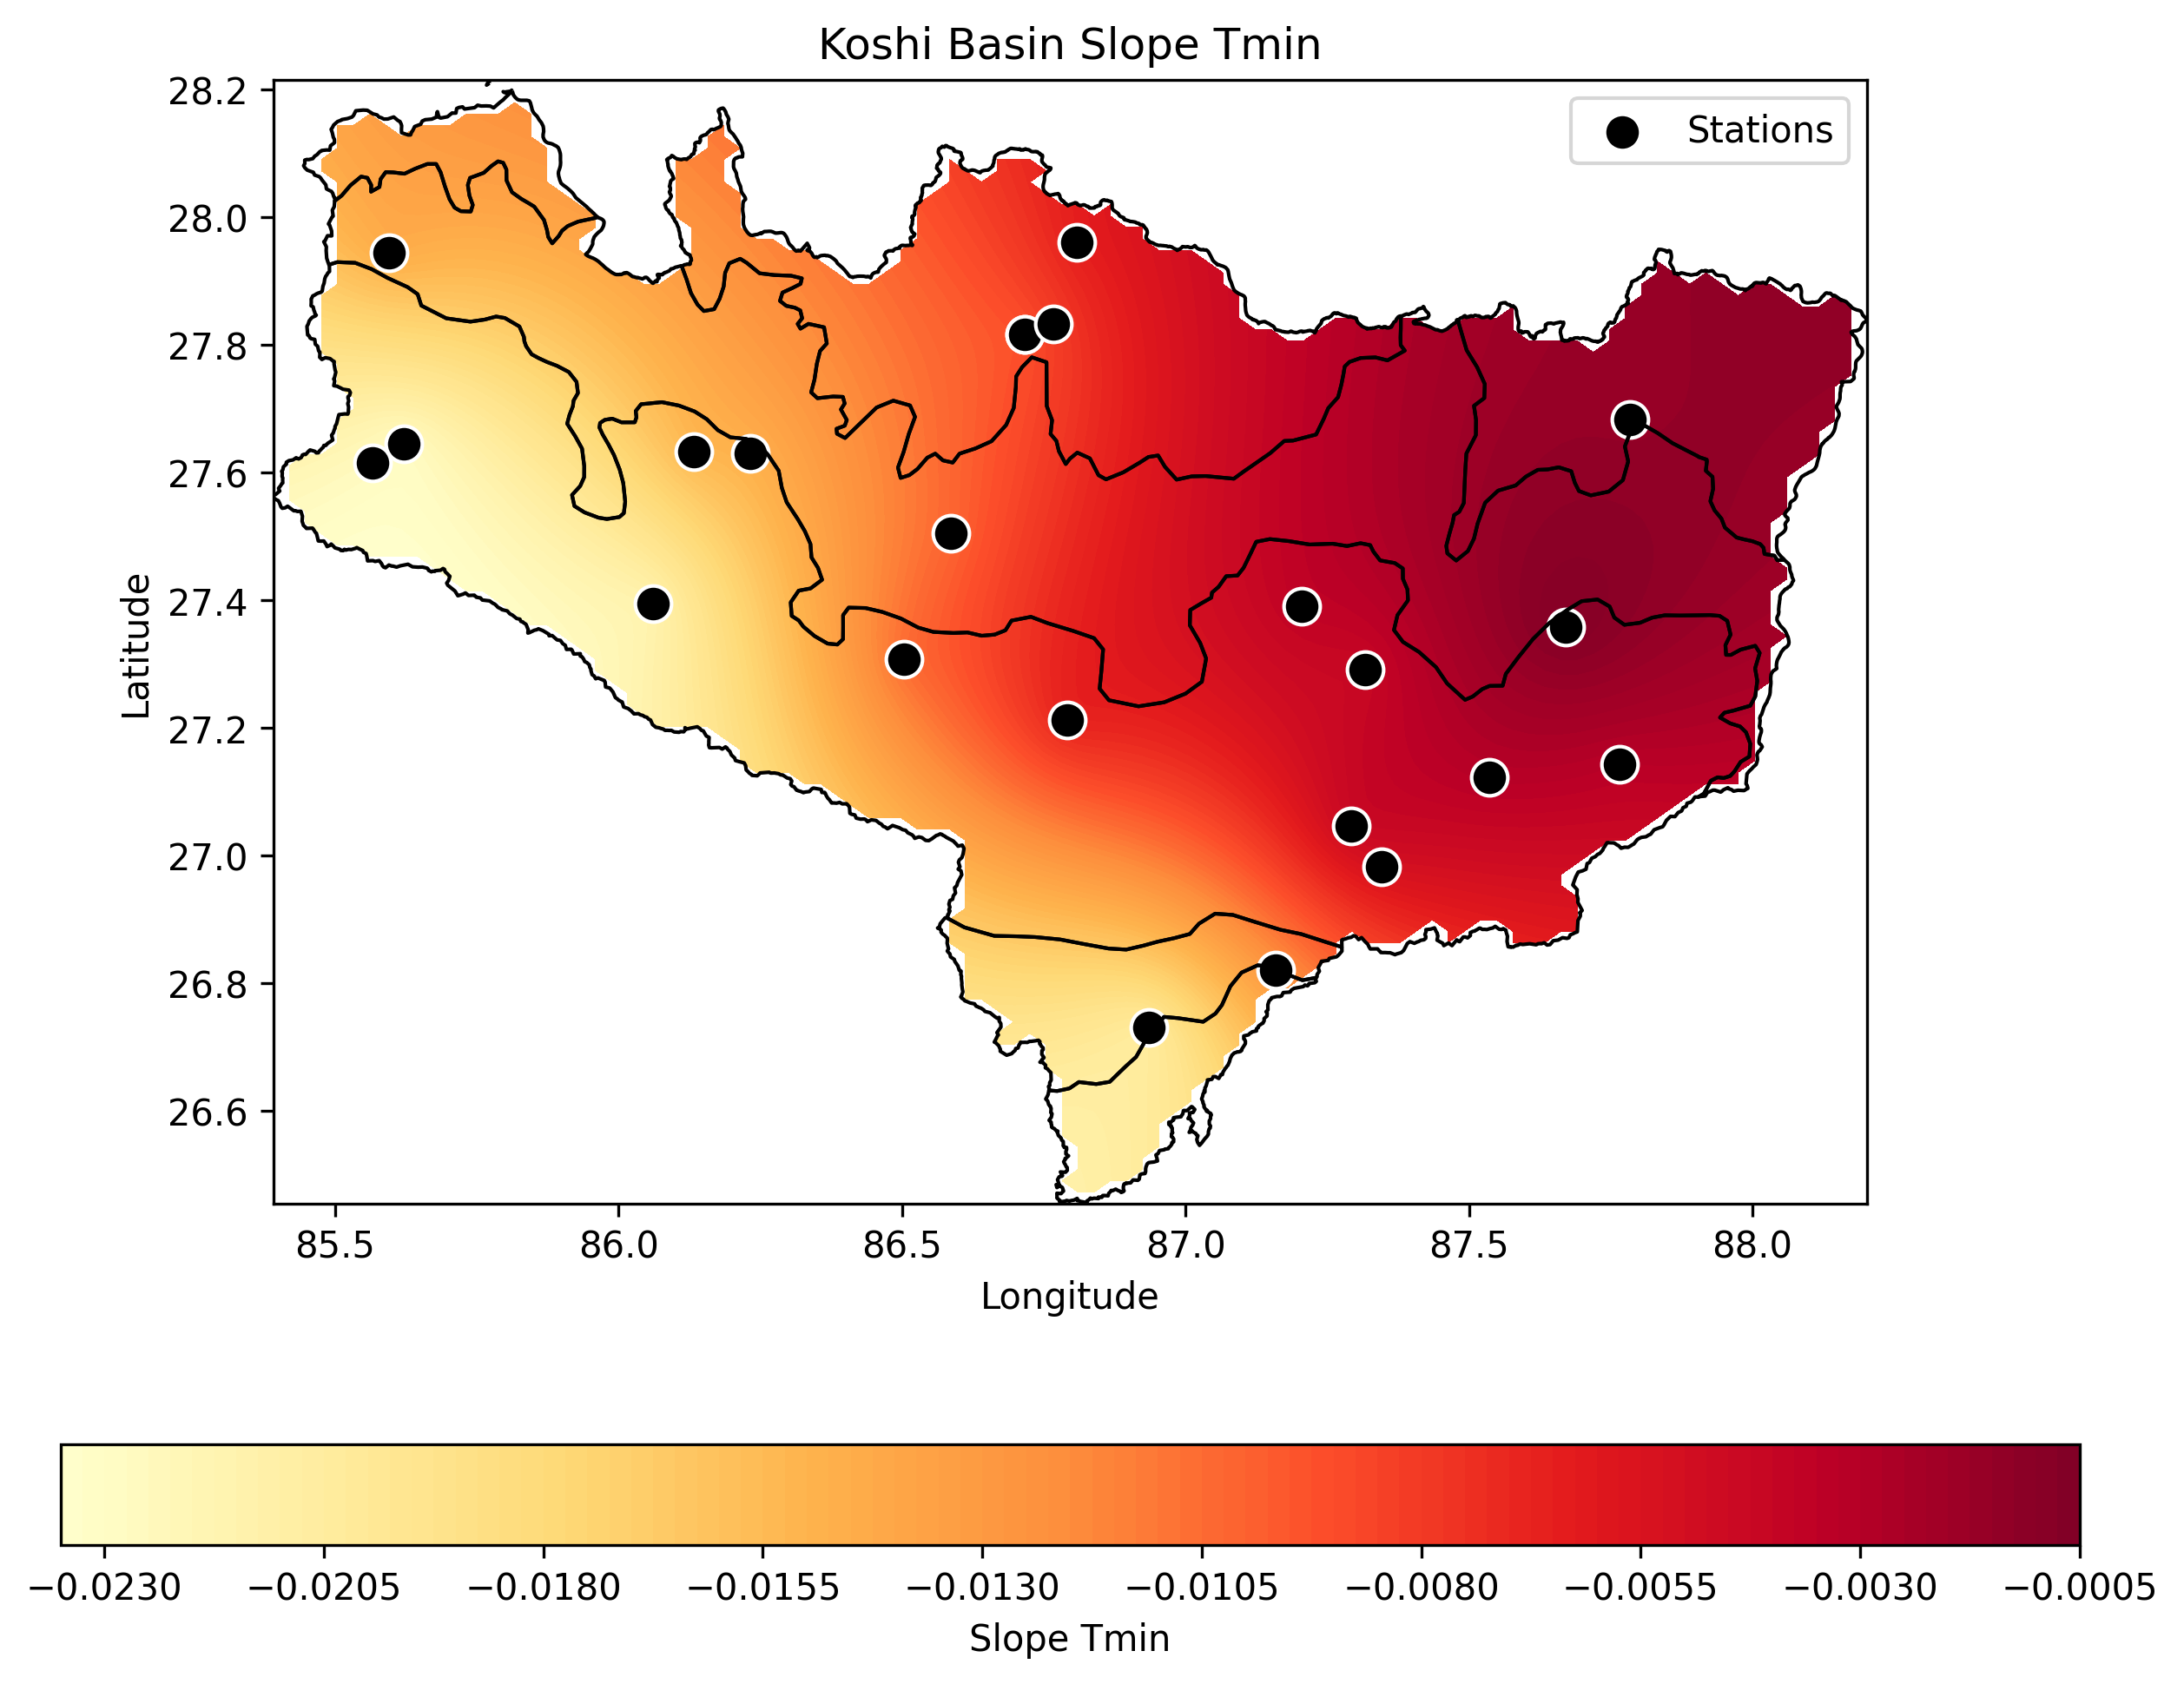
\includegraphics[width=\linewidth]{images/avg_krig_Koshi Basin Slope Tmin.png}
      \caption{Minimum Temperature Trend}
      \label{fig:basin_min_trend}
  \end{subfigure}
  \hfill
  \begin{subfigure}{0.45\textwidth}
      \centering
      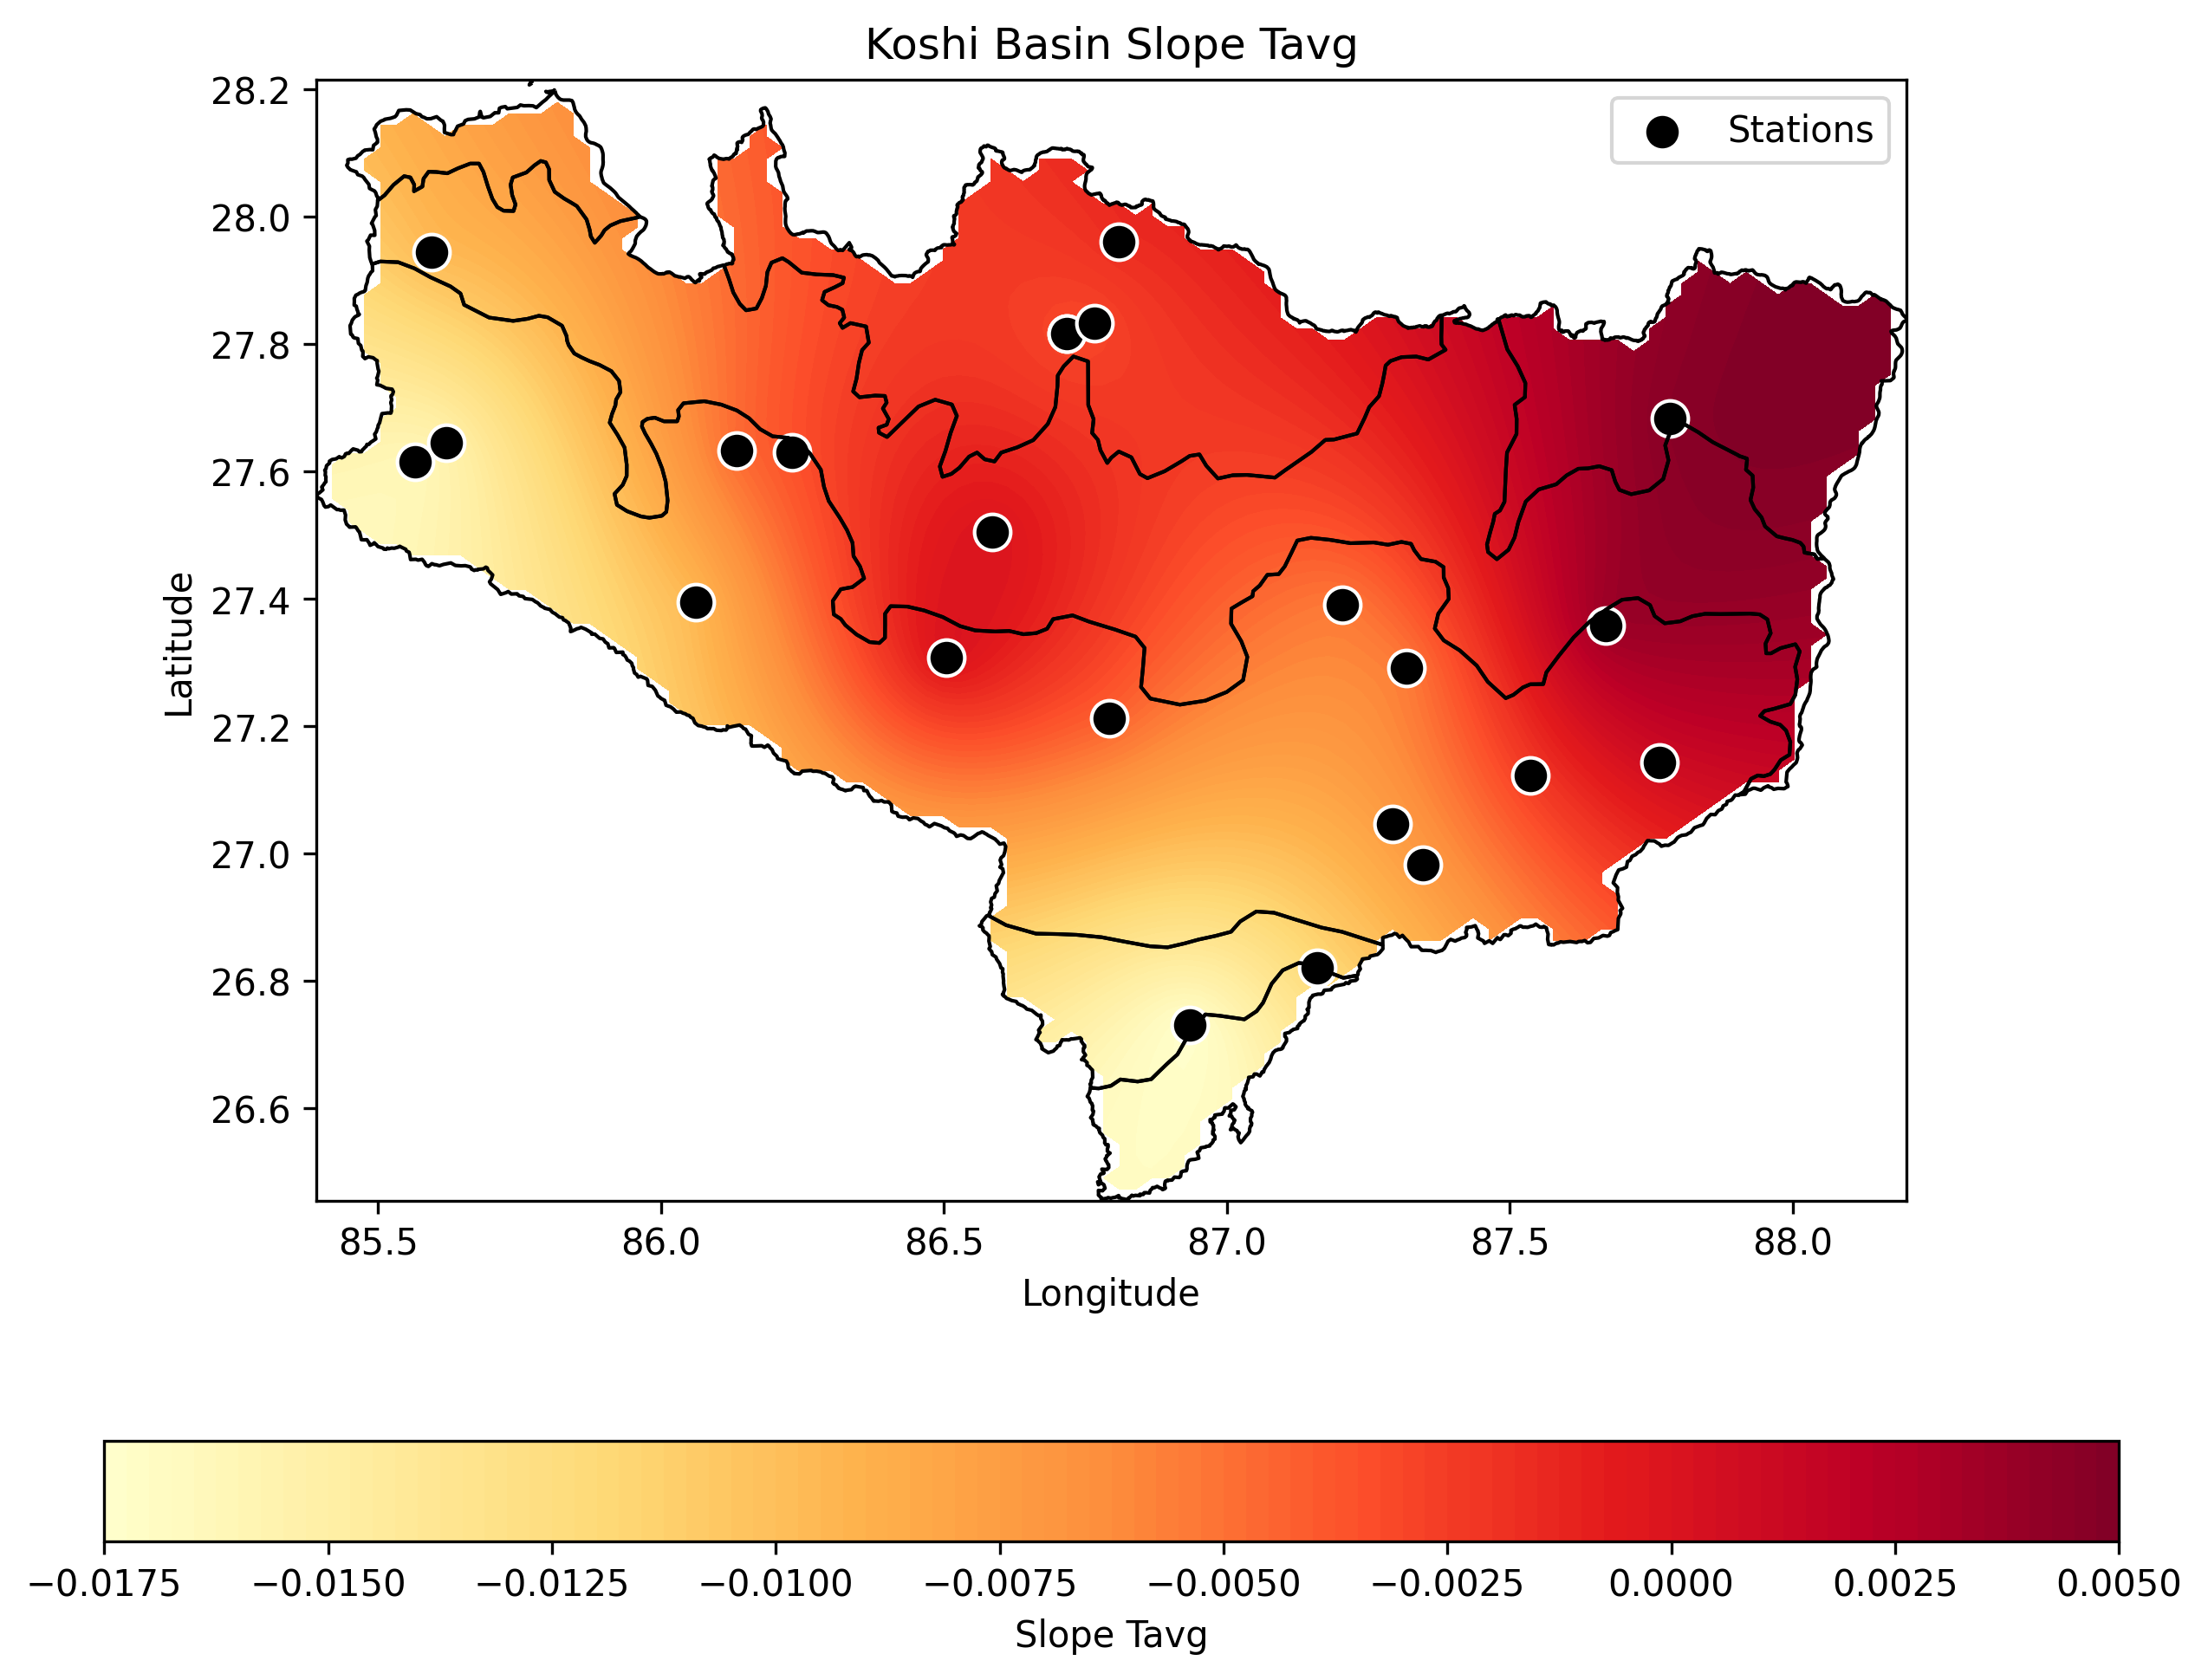
\includegraphics[width=\linewidth]{images/avg_krig_Koshi Basin Slope Tavg.png}
      \caption{Average Temperature Trend}
      \label{fig:basin_avg_trend}
  \end{subfigure}
  
  \vspace{0.5cm} % Adjust space between rows as needed
  
  \begin{subfigure}{0.45\textwidth}
      \centering
      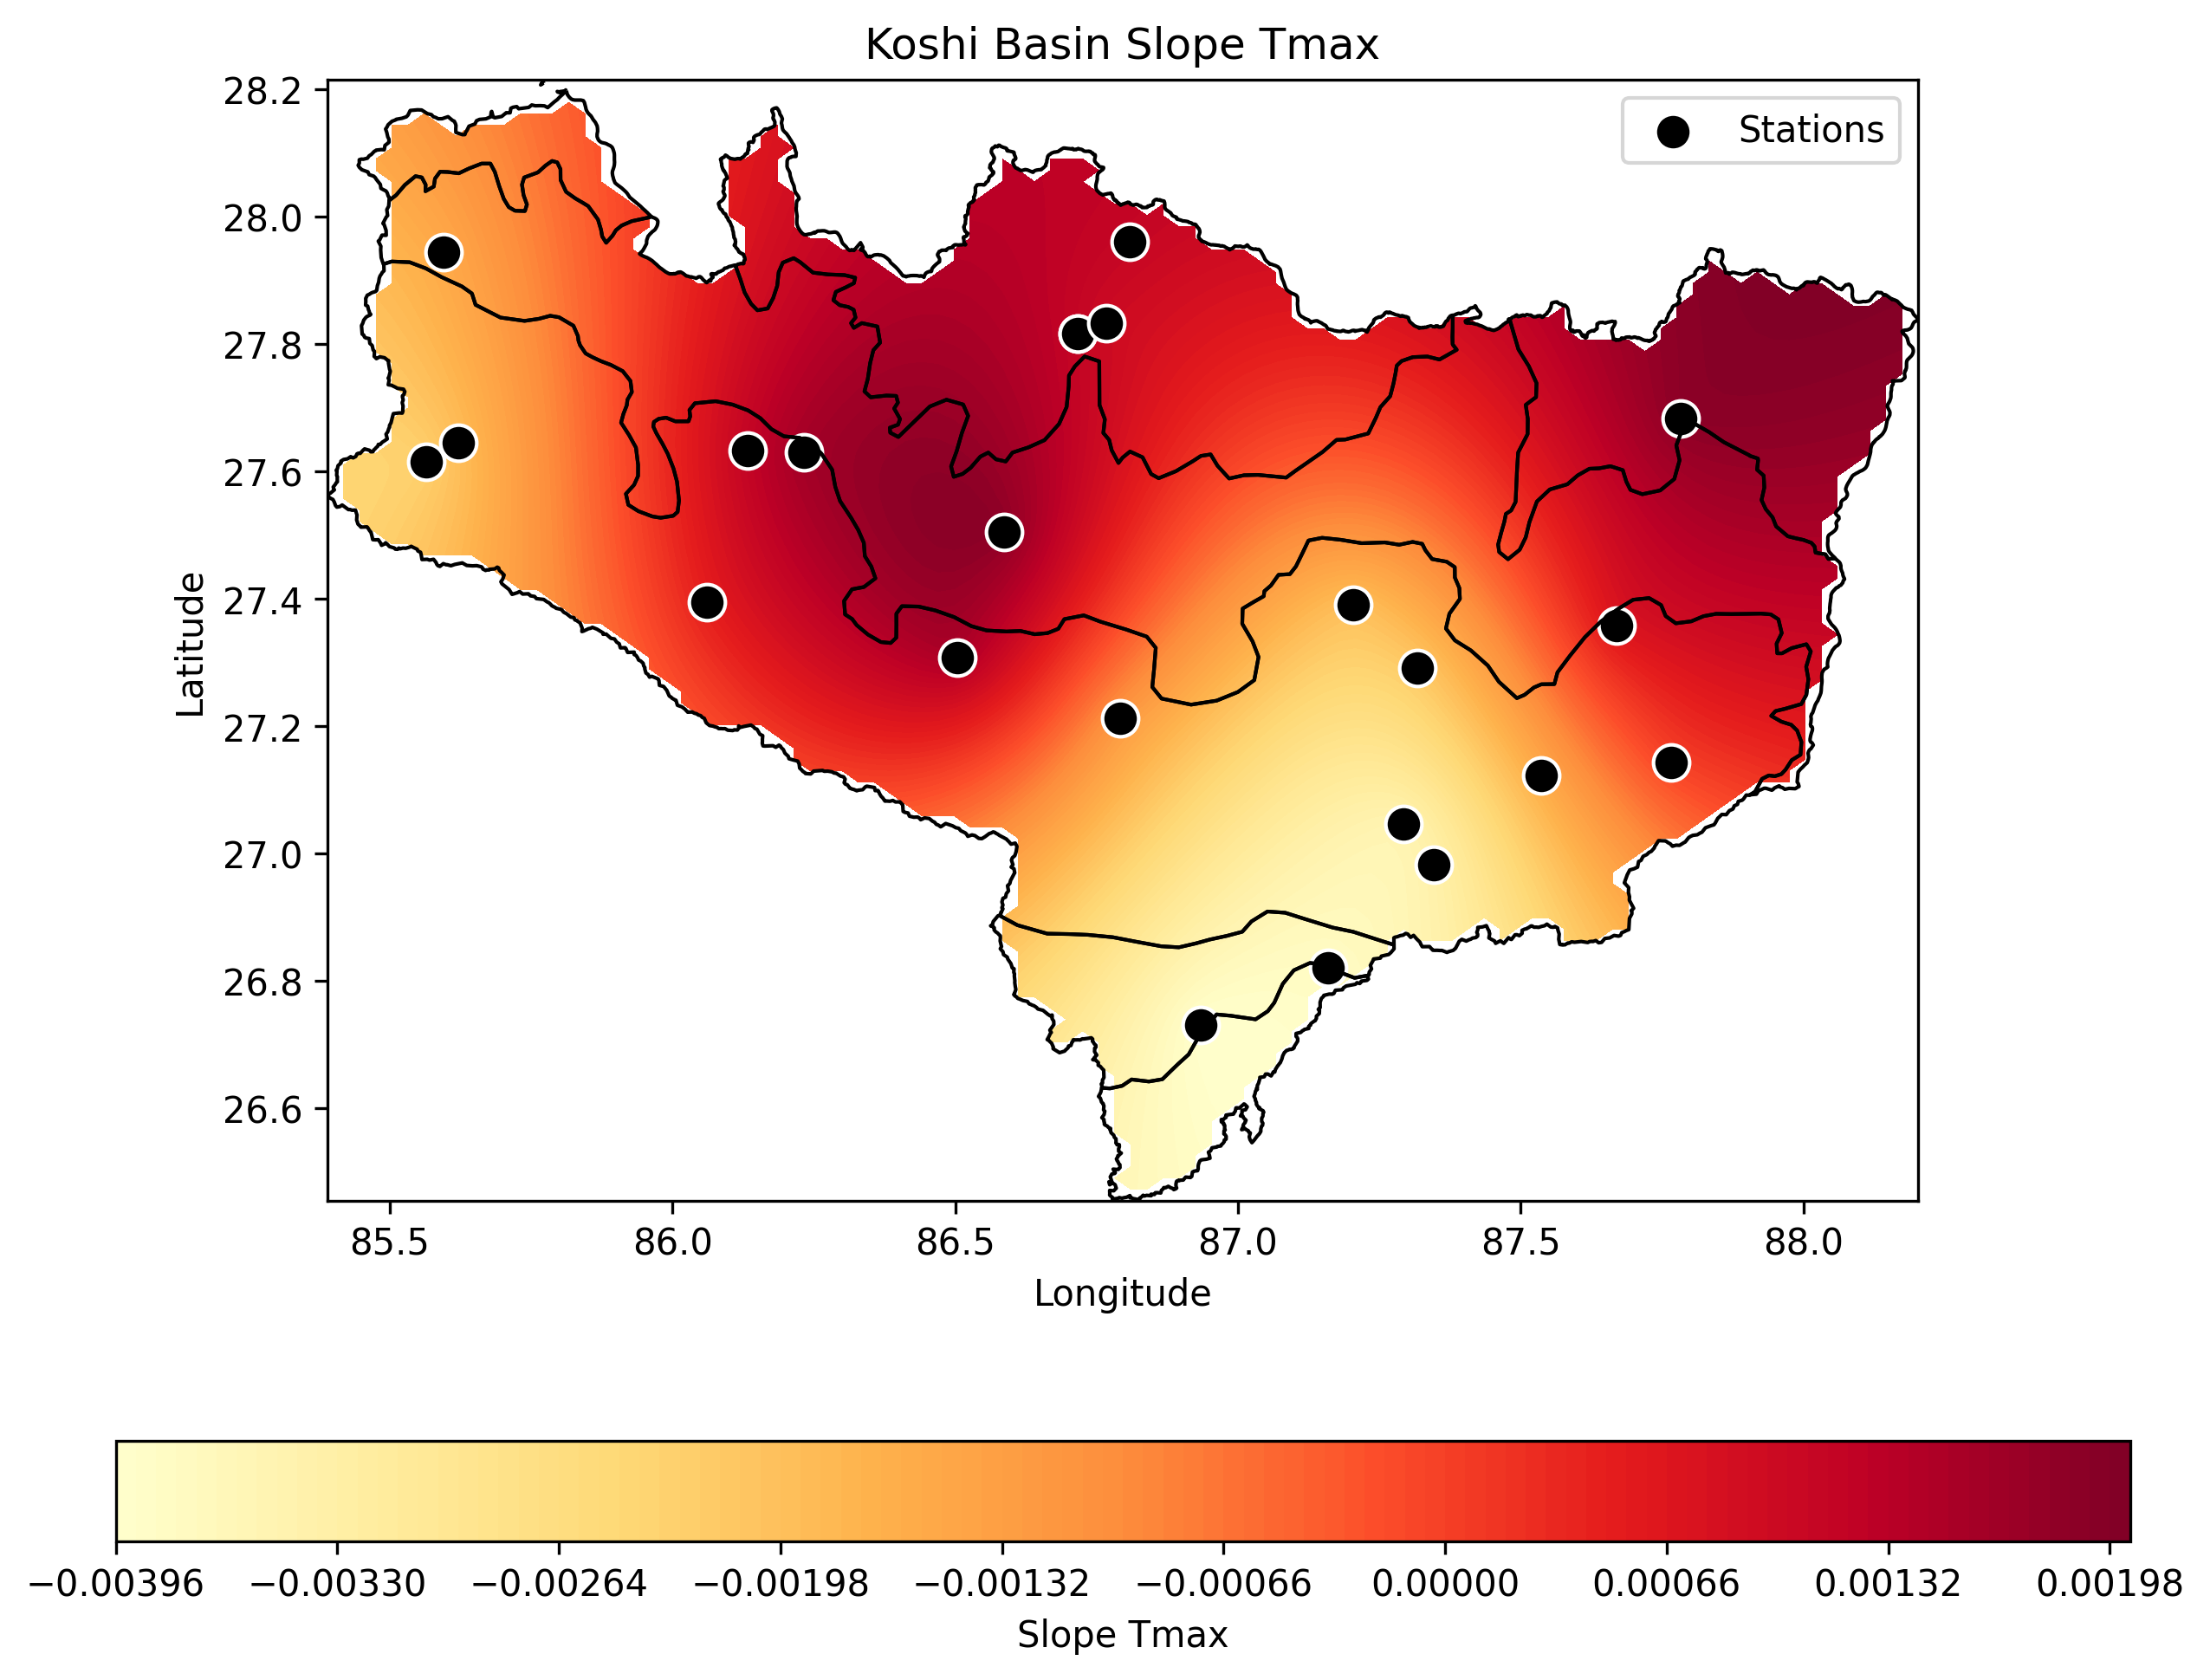
\includegraphics[width=\linewidth]{images/avg_krig_Koshi Basin Slope Tmax.png}
      \caption{Maximum Temperature Trend}
      \label{fig:basin_max_trend}
  \end{subfigure}
  
  \caption{Spatial distributions of annual temperature trends for the period 1962–2022 for (a) Tmin, (b) Tavg, (c) Tmax}
  \label{fig:krig_results}
\end{figure}

The results obtained from the analysis reveal a heterogeneous temperature trend across the Koshi basin region, as illustrated in Figure \ref{fig:krig_results}. An annual average of daily minimum temperatures shows an overall cooling trend, as shown in Figure \ref{fig:basin_min_trend}, ranging from -0.0005°C to -0.023°C, with higher elevations experiencing less cooling. As shown in Figure \ref{fig:basin_avg_trend}, the annual average temperatures reveal both warming and cooling trends, ranging from -0.0175°C to 0.005°C, where higher elevations tend to warm or cool less, when compared to the Tarai and Siwalik regions. Similarly, the annual average of daily maximum temperatures shows trends from cooling to slight warming (Figure \ref{fig:basin_max_trend}), ranging from -0.00396°C to 0.00198°C, with Tmax exhibiting a warming trend in higher elevation areas. Study conducted by Paudel et al. (2021) in transboundary Koshi basin for the years between 1980 and 2018, revealed an increase in the mean annual temperature by 0.084°C/ year in the mountain region (p = 0.0005), by 0.0975°C/year in the hill region (p = 0.0002), and by 0.0187°C/year in the Tarai region (p = 0.0206), with significant correlations throughout. 

\textcite{adhikari_x_2016} studied temperature trends from 1988 to 2010 in the Annapurna, Langtang, and Khumbu regions of Nepal. In the Khumbu region, moderate warming was observed across all seasons, with maximum temperatures rising by 0.0857°C/year in winter and 0.0628°C/year in pre-monsoon. The trend in the change of minimum temperatures was slightly different with a small increase of 0.0101°C/year in spring and a decrease of -0.0024°C/year during monsoon. Overall, mean temperatures increased by 0.0857°C/year in winter, with Khumbu showing lower trends compared to Langtang and Annapurna, particularly in minimum temperatures.





\section{Summary}
this is conclusion \citet{intergovernmental_panel_on_climate_change_ipcc_climate_2023} .

\section*{References}
\printbibliography
\end{document}
